%\documentclass[11pt,dvipdfm]{article}
\documentclass[11pt]{article} %The above line must be used for your camera-ready submission, which requires a latex -> DVI -> PDF compilation pipeline.  As a workaround while you are writing your paper, you could comment it out and use this line instead, which is compatible with pdflatex.
\usepackage{deauthor,times,graphicx,hyperref}
\usepackage{wrapfig}
\usepackage{amssymb}
\usepackage{graphics}
\usepackage{xcolor}
\usepackage{pifont}
%\usepackage{subcaption} % for subtable
\usepackage{subfigure}
\usepackage{booktabs} % for tables
\usepackage{threeparttable} % for tablenotes

\newcommand{\cmark}{\ding{51}}%
\newcommand{\xmark}{\ding{55}}%



\begin{document}
\title{Social Media Data - Our Ethical Conundrum}


\author{Lisa Singh, Agoritsa Polyzou, Yanchen Wang, Jason Farr, Carole Roan Gresenz\\Georgetown University\\ \{lisa.singh, ap1744, yw516, jaf301, carole.roan.grensenz\}@georgetown.edu}


\maketitle
\begin{abstract}
Our field is engaging more and more in the development of algorithms, models, and technologies to better understand human demographics, opinions, and behaviors. These data range from product and movie reviews to opinions about issues of the day. While we have begun to grapple with some ethical issues associated with using these data, we may still be ignoring, or at least underestimating, the ethical complexities related to the computational tasks we work on, the data we use, and the technologies we create. This paper focuses on the challenges associated with using social media data and the ethical considerations these challenges create. We frame the ethical dilemmas within the context of data privacy and algorithmic bias (fairness) and show how and when different ethical concerns arise. A recurrent theme throughout is the lack of transparency. Therefore, we conclude by suggesting a need exists to consider transparency throughout the software development lifecycle and develop mechanisms that incorporate ideas related to transparency as part of the foundation of human-computer systems. By cataloging these complexities and their ethical considerations, we hope that our field pauses and thinks through these issues as we continue to build algorithms and tools for social media. 

\end{abstract}

\section{Introduction}
\label{intro}
As a society, we generate massive amounts of data about different aspects of our lives. We share our opinions on movies and products, our beliefs about religion and politics, and our day to day actions and movement patterns with tens of apps and online platforms. At the same time, the cost of large-scale computing infrastructures continue to decrease, allowing for corporations and researchers to build sophisticated algorithms that model human behavior and opinion at scale. Much research has emerged about how companies and researchers are using these data without regard for ethical norms or traditional research integrity standards~\cite{Kramer8788,10.1177/1747016117738559,samuel2019}. A 2020 movie, the Social Dilemma, details how algorithms are being used to manipulate users and change their behavior, even in cases where the change may not be healthy \cite{socialdilemma}. Together, these different avenues remind us how users who share data online are being exploited. 

As computer scientists, we are trained to collect whatever data are available to develop database systems or data mining, machine learning, and natural language processing (NLP) algorithms. Because our focus is the development of novel algorithms and innovative technologies as opposed to behavioral or social research, we are not taught to view \textit{data} as \textit{human} data. In contrast, protection of human subjects is the cornerstone of social science and medical/public health research. Toward that end, many social scientists use survey instruments to measure different constructs of interest. These surveys require that participants consent, and participants know exactly how the data from the study will be used, stored, and for how long. With social media data, companies and researchers can access data without the traditional human subject safeguards in place. Unfortunately, because computer scientists are broadening their research objectives and delving into creating algorithms and tools to model and learn human behavior~\cite{Kramer8788,fb_Analytica}, we can no longer ignore our connection to human data or the impact our creations have on society. As the era of machine-driven intelligence begins, ethical considerations must become front and center for computer scientists using social and behavioral data, and be part of the foundation of data-centered computer science. 

To help reach this goal, this paper takes a look at ethical challenges associated with using social media data. There are many reasons to focus on social media data. First, these data are much more readily accessible to companies and researchers than many other forms of data. Second, norms on different platforms lend themselves to different ethical concerns that need to be explored \cite{ozkula2020}. Finally, the potential for harm to individuals (or society more broadly) is enormous, ranging from misrepresentation of attitudes and opinions to loss of reputation, and even discrimination and manipulation \cite{10.1080/15265161.2019.1602190,Susser2018, kammourieh2017, luka2017}. 

A number of ethical frameworks have been developed, including bioethics \cite{Turoldo2008,TANGWA2009S2}, computer ethics \cite{10.1145/3376898}, and big data ethics \cite{7515114,Lipworth2017}.  In this paper, we begin by using this literature to define a set of relevant ethical principles. We then consider them in the context of data privacy and algorithmic bias, focusing our discussion on those that are most relevant to social media. The crux of this paper identifies complexities associated with using social media data, describes the complexities, provides context for these challenge on some well known social media platforms, and then maps the ethical considerations to these social media complexities in the context of data privacy (Section \ref{sec:privacy}) and algorithmic bias (fairness) (Section \ref{sec:bias}).  As part of our discussion, we show how these challenges manifest themselves across six popular platforms: Facebook, Instagram, Snapchat, Tiktok, Twitter, and LinkedIn. Our hope is that, as a field, we move away from ignoring the ethical realities of the data we use. Data privacy and algorithmic bias connect to some of the ethical principles we define, but not all of them, particularly with regards to transparency. Therefore, considering a new area of research focused on transparent computing (Section \ref{sec:transparency}), in which principles of informing users about decisions throughout the computational lifecycle is a central design consideration, would help further embed ethical principles within computer science. This idea goes beyond transparency of model to transparency of the human-computer system.

\section{Ethical principals relevant to social media}
\label{sec:ethics}

Building off of the previous literature \cite{ozkula2020,b88a5a9441354a02ac5b105291fff917,10.1177/1556264619901215,10.1080/15265161.2019.1611278,us1979belmont}, Figure~\ref{fig:ethical-pillars} identifies a basic set of ethical principles associated with moral responsibility. \textit{Non-maleficence} is the responsibility to refrain from causing harm. This principle is especially relevant in cases where the use of data might negatively affect children or participants with mental health issues. \textit{Beneficence} directs researchers to offer kindness or other benefits to participants, wherever appropriate and possible. In rare cases, for example, a researcher might come across social media posts that indicate a participant is in need of immediate intervention. Together, beneficence and non-malfeasance concern the positive and negative impacts on the participants of the study. \textit{Maximizing social benefit} concerns the broader, societal impacts of the study, including whether the research adds value or improves society or research understanding. While computer science research has added value and improved society in many ways, societal benefit is not emphasized as a foundational tenet of computer science research. \textit{Respect for autonomy} requires that researchers allow potential participants to choose their own actions, including whether to participate in the study and what data (if any) to share. Researchers should explain the details of the study to participants and, as a general rule, refrain from any sort of manipulative practices that would covertly undercut the decision-making faculties of the participant. \textit{Justice} focuses on ensuring that the study does not discriminate against subpopulations or increase inequities, and that subpopulations are not at risk of being excluded from possible benefits. Justice also includes clear justification of the value of the research and transparency of the research protocol. Finally, \textit{proportionality} focuses on ensuring that better ways do not exist for conducting the study that may be less invasive or more equitable. While many other ethical principles exist, these ones are particularly important in the context of social media data.

\begin{figure}[tb]
	\centering
        %	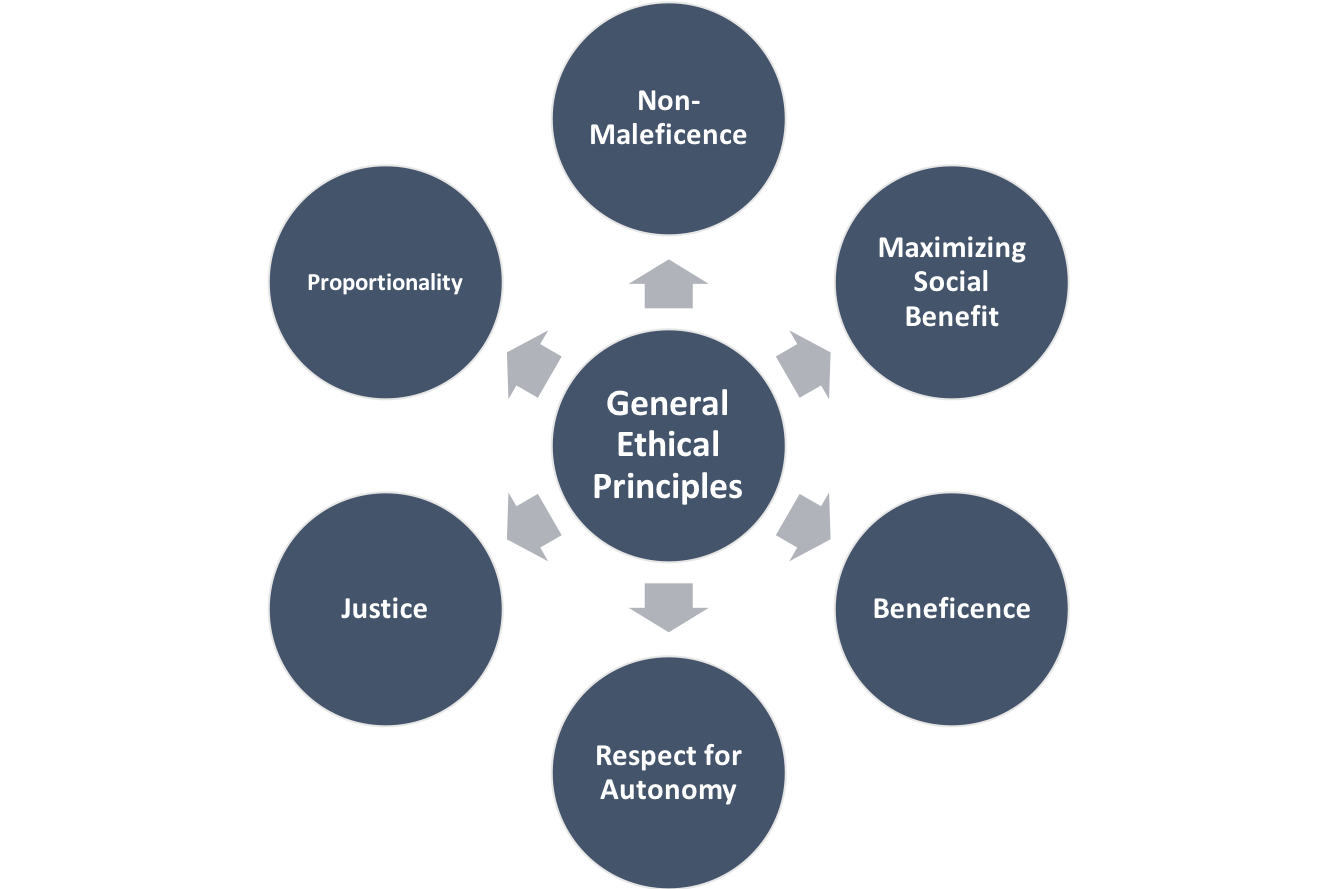
\includegraphics[width=0.5\textwidth,natwidth=850,natheight=550]{figs/ethical-pillars3.png}
        	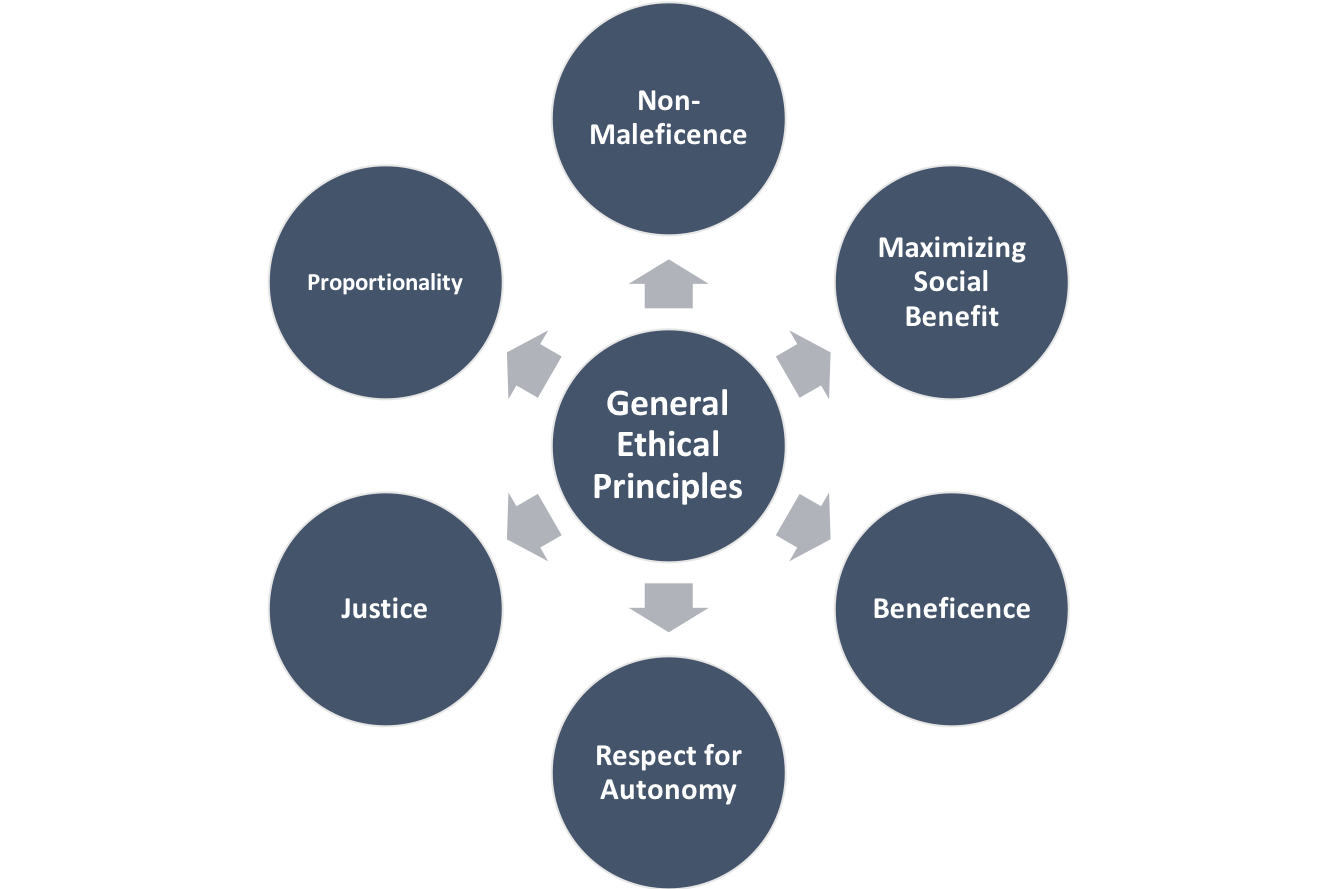
\includegraphics[width=0.5\textwidth]{figs/ethical-pillars3.png}
	\caption{Ethical Principles Applicable to Social Media Setting}
	\label{fig:ethical-pillars}
\end{figure}

Researchers in computer science already make choices in the ordinary course of their studies that draw upon these ethical principles.  Non-maleficence, beneficence, and justice are core principles used to define measures of fairness in machine learning and algorithmic bias. Respect for autonomy and proportionality are foundational concepts within data privacy. Connecting to society and maximizing social good have become themes within subareas of computer science, e.g. data science for social good and AI for social good. As we continue to understand computer science research within the context of different ethical complexities, we must consider harm caused by both processes and entities creating and using developed technologies. Processes include the use of algorithms and models that are biased, lack transparency, or reduce privacy. Measuring algorithmic bias and data exposure are two ways to understand the harm caused by processes. Entities include companies (data collectors), researchers and others (data utilizers) who make decisions that can cause harm to individuals (data generators) or reduce societal benefit. Understanding the role that different entities play in decision making can help researchers better understand their ethical responsibilities when using these types of data. 

\section{Challenges and Foundations}
\label{sec:notation}
Social media challenges are generated by design decisions of each platform, by the types of data users share publicly and privately, and/or the different way researchers and other external groups use the data. Figure \ref{fig:framing} identifies some of these challenges and places them in the context of data privacy and algorithmic bias. In Sections \ref{sec:privacy} and \ref{sec:bias} we will go through these challenges in more detail. 

To start the formalization around some of the concepts we will use, we propose the following mathematical framing of the social media challenges and ethical principles. We will use a security threat model perspective, where an \textit{attack} occurs when ethical considerations are ignored. Let $\mathcal{S} = \{s_1, s_2, \ldots, s_k\}$ be social media sites (platforms). For each social media site, $s_i \in \mathcal{S}$, let $\mathcal{I}_i=\{\mathcal{G}_i, \mathcal{B}_i\}$, where $\mathcal{G}_i = \mathcal{G}^p_i \cup \mathcal{G}^h_i$ is the set of attributes provided by the user and those attributes can be public $\mathcal{G}^p_i$ or hidden $\mathcal{G}^h_i$ and $\mathcal{B}_i$ is the set of attributes auto-generated by  $s_i$. Examples of attributes in $\mathcal{G}_i$ are the user's name and date of birth, while examples of auto-generated attributes in $\mathcal{B}_i$ include the number of friends/followers. Let $\widetilde{\mathcal{I}}_i = \{\widetilde{\mathcal{G}}_i, \widetilde{\mathcal{B}}_i\}$ be the attributes shared by the platforms other than $s_i$, i.e., $\mathcal{S} - \{s_i\}$. 

We define the set of users as $\mathcal{U} = \{u_1, u_2, \cdots, u_n\}$, and define $c(u_j)$ to be a  user class or group that $u_j$ belongs to based on his/her sensitive attributes. User $u_j$ must provide some information when registering on platform $s_i$. The information includes both required and optional fields in  $\mathcal{G}_i$. We denote the user's information as $\mathcal{G}_{i,j}$, and by definition it corresponds to some or all of the attributes captured by platform $\mathcal{G}_i$. 

Social media platforms can use user information to predict values about users. Let $f_i:\mathcal{G}_i \cup \widetilde{\mathcal{G}}_i \rightarrow \mathcal{L}_i$ be a function or model built by social media site $s_i$ which uses information provided by the user $\mathcal{G}_{i,j}$ on $s_i$ and other user information shared by other sites $\widetilde{\mathcal{G}}_i$ to make inferences. $\mathcal{L}_i$ represents attributes learned or inferred by different entities, including social media site $s_i$, and $\mathcal{L}_{i,j}$ are the attributes values inferred for user $u_j$. 

Fundamentally, our security goals are to maintain user privacy, ensure fairness towards individual users $u_j \in \mathcal{U}$ or group of users determined by $c(\cdot)$ (nondiscriminatory behavior), and help users make informed decisions (through transparency). These goals can be mapped to the ethical principles we want to adhere to that were presented in the previous section. There are multiple adversaries in this framing, including social media platforms and other companies $S$, researchers $R$, and other platform users $\mathcal{U}-\{u_j\}$. Let $\mathcal{A}$ be the set of all adversaries, $\mathcal{A} = \mathcal{S} \cup \mathcal{R} \cup \{ \mathcal{U} - \{u_j\} \}$. At a basic level, an adversarial attack occurs when any entity $a \in \mathcal{A}$ uses information in $\mathcal{I}_i$ or $\widetilde{\mathcal{I}}_i$ or $\mathcal{L}_i$ to \textit{violate} one or more of our ethical principles, $\mathcal{E}$. We use the term violate to mean that the ethical consideration is being ignored and/or the expectations of users, in general, are not being met -- a `line' is being crossed.\footnote{This could be modeled as an allowable budget for each ethical consideration.} Let $g: \mathcal{I}_i \cup \widetilde{\mathcal{I}}_i \cup \mathcal{L}_i \rightarrow \mathcal{E}$ be a function that $a_j$ uses to build a model violating ethical principles in $\mathcal{E}$. 

\begin{figure}[tb]
    \centering
    %    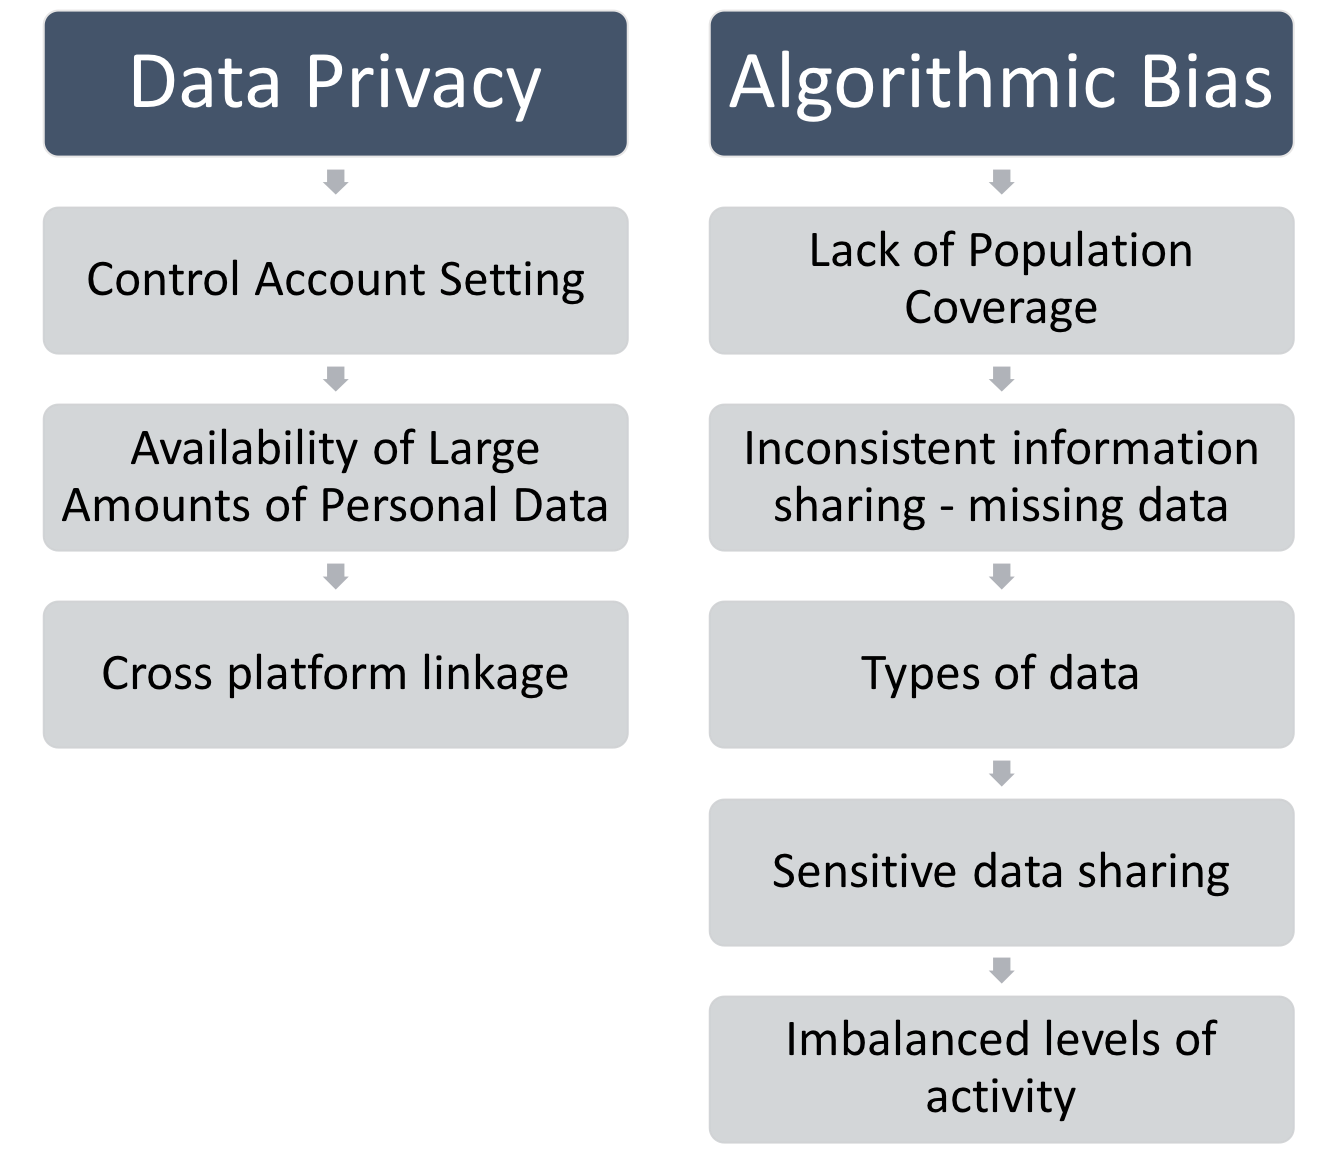
\includegraphics[width=0.35\textwidth,natwidth=890,natheight=730]{figs/sm-challenges2.png}
        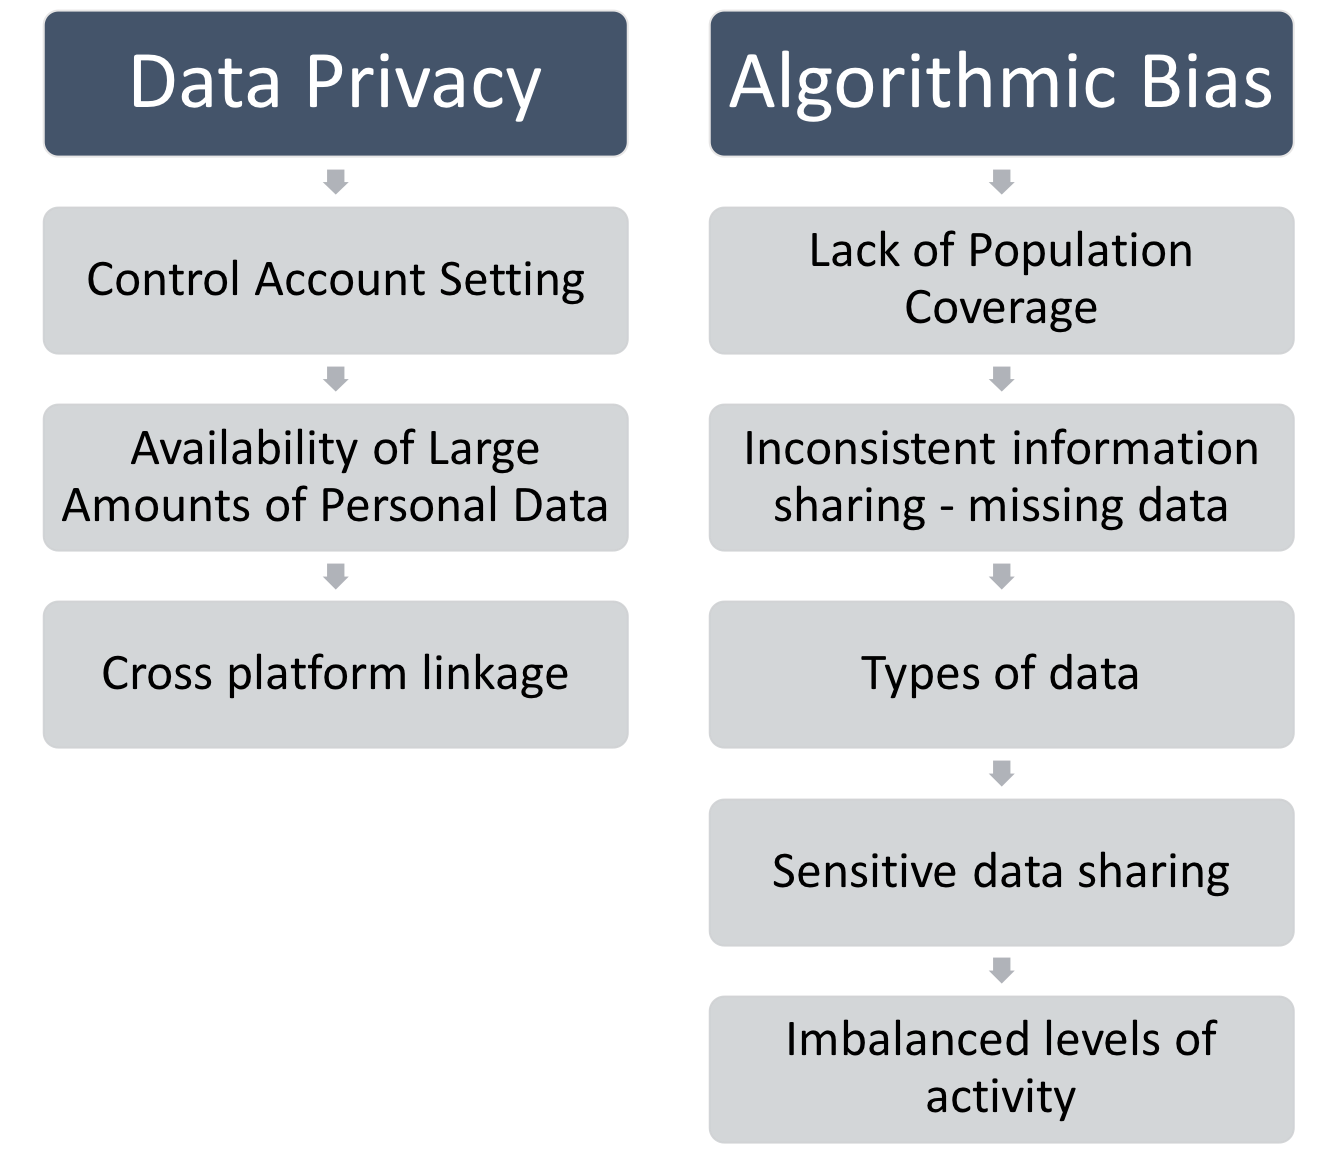
\includegraphics[width=0.35\textwidth]{figs/sm-challenges2.png}
    \caption{Social Media Complexities Within the Contexts of Data Privacy and Algorithmic Bias}
    \label{fig:framing}
\end{figure}
\section{Data Privacy} 
\label{sec:privacy} 
Data privacy research focuses on measuring and reducing the amount of sensitive information that is disclosed. Within the context of social media data, particular attention needs to be paid to disclosure during data collection and data processing. One goal of data privacy research is to develop models and tools that allow users control over their data (and who can access them) and protect each user's privacy preferences and personally identifiable information. Data privacy is a challenging task and it has an even more complicated framing when examined on social media.
For example, social media users freely share large amounts of data that may leak unintended information.  Spontaneous posts and reactions could give insight into sensitive information. Social media companies collect thousands of data points about users, including their photos, their friends, their likes, their activity on the platform,  pages they visit, online purchases, contacts list, and even their location. According to a recent study~\cite{bagrow2019}, advertisers can profile someone with 95\% accuracy using the information from just eight or nine of their friends’ social media accounts. 

Challenges with regards to social media and data privacy arise because users share large amount of information and they have little control over how it is used. This leads to concerns around respect for autonomy, justice proportionality, and maximizing societal benefit.

\subsection{Ability to Control Account Setting}
From an ethical perspective, users should have control of the information they choose to share with the public and with the social media platform. So when an account is setup on a platform, the default setting should always be private ($\mathcal{G}^p_i = \emptyset$ and $\mathcal{G}_i = \mathcal{G}^h_i$), allowing users to make parts of their account public if they choose. They should also not be required to share sensitive information with the platform in order to setup an account. Unfortunately, to promote public discussion and increase community, the default approach for most social media platforms is to setup user accounts as publicly accessible by anyone using the platform, and ask for some sensitive pieces of information during registration. For our example companies, five of the platforms setup public user accounts by default (Snapchat is the one exception). From previous research, we know that part of the reason for this default public setting is that people are not overly concerned with privacy \cite{madden2013teens,SENTHILKUMARN2016114}. Even though concern has risen in recent years \cite{smconcern,smconcern1}, most users do not change their privacy settings to be more private, bringing rise to the ``privacy paradox''~\cite{kokolakis2017,barth2017}. These privacy settings define which features belong to $\mathcal{G}^p_i$ and which to $\mathcal{G}^h_i$, and how successful attacks conducted by adversaries in $\mathcal{A}$ can be.

Given that five of these six platforms are public by default, we begin by trying to understanding how publicly visible user generated data are, what types of information are visible, and whether or not users can make all the publicly visible information private. Table \ref{tab:privacy_setting} summaries the ability of users to control their privacy settings. We organize the table by the subgroup that generates the data fields and the typical functionality on platforms. Users share their data, e.g. account information. Other users ($\mathcal{U}-\{u_i\}$) on the platform can share information about a user $u_i$, e.g. tagging a photo. The last subgroup is about auto-generated fields and platform functionality that expose users information. The table shows that platforms give users control over the data they provide and what other users can do with respect to their data. This is important progress for our industry and likely a result of recent legislation in Europe. However, some platforms fail to let users make data that are generated by the platform private (Twitter, Tiktok, LinkedIn, and Instagram). For example, Twitter users cannot hide their number of followers on their profile page, and LinkedIn users cannot hide their number of connections. 
Platforms sometimes also require users to use functionality that makes use of their shared data. As an example, Instagram does not allow users to turn off personalized ads. 



\begin{table}[]
\caption{Users ability to control their privacy settings}
\label{tab:privacy_setting}
\resizebox{\columnwidth}{!}{%
\begin{tabular}{l lcccccc}
% \begin{tabular}{l lc|c|c|c|c|c}
\toprule
\textbf{Data Generators}                         & \textbf{Data Fields}                                  & \textbf{Facebook} & \textbf{Instagram} & \textbf{Snapchat} & \textbf{Tiktok} & \textbf{Twitter} & \textbf{LinkedIn} \\ \midrule
Individual                       & Profile/account information  & \cmark    & \cmark     & \cmark    & \cmark  & \cmark   & \cmark    \\ \cline{2-8} 
users                          & Posts/story                   & \cmark    & \cmark     & \cmark    & \cmark  & \cmark   & \cmark    \\ \midrule
Other users                        & Tag/mention user             & \cmark    & \cmark     & N/A      & \cmark  & \cmark   & \cmark    \\ \cline{2-8} 
             & Contact user / send comment     & \cmark    & \cmark     & \cmark    & \cmark  & \cmark   & \cmark        \\ \midrule
Platform                        & Personalized ads                       & \cmark    & \xmark     & \cmark    & \cmark  & \cmark   & \cmark    \\ \cline{2-8} 
                & Auto-generated fields                    & \cmark    & \xmark     & N/A      & \xmark  & \xmark   & \xmark    \\ \cline{2-8} 
                        & External partner data sharing                           & \cmark    & \xmark     & \cmark    & \cmark  & \cmark   & \cmark \\ \cline{2-8} 
                        & User search                & \cmark    & \cmark     & \cmark    & \cmark  & \cmark   & \cmark \\ \bottomrule
\end{tabular}%
}
\end{table}


In this context, the two fundamental data privacy concerns are that accounts are public by default ($\mathcal{G}_i \neq \mathcal{G}^h_i$), and not all data fields can be hidden ($\mathcal{G}^p_i \neq \emptyset$). Also, sites are unclear about their default settings or how to change them (lack of transparency).
One problem that arises specifically for researchers and other data utilizers is that some of the data are private, and using the private data for research without user consent can be violate the principles of respect for data ownership and maintenance of privacy. Together, the ethical dilemmas arising from this social media challenge are justice, respect for autonomy, and proportionality. Justice because it is likely that there are subgroups who are structurally speaking more likely not to understand the privacy settings, the defaults, etc., and are therefore, more vulnerable to the manipulation that can occur when the default settings offer no privacy. 
Autonomy is not respected because the default lack of privacy means more data about the users are available to manipulate them through targeted advertisements (commercial, political, or otherwise)~\cite{Susser2018}. Finally, issues of proportionality arise because companies are not being transparent about the default settings or how to change them, leading to more invasive usage of human data and less equitable treatment.
 


\subsection{The Availability of Large Amounts of Personal Data}
Users make decisions about the data they want to share or not share. Figure \ref{fig:req_fields} shows the basic information users need to share to open an account on our example platforms as of November 2020. All the platforms require an email or phone number to register. We see that the number of required fields ranges from three (Twitter) to six (LinkedIn). Five of the six platforms require birthdate (LinkedIn is the one exception), a piece of sensitive information. These required fields along with user activity/post data become the basis for auto-generated fields that lead to 1000s if not 100,000s of new data points for companies. 

%\begin{table}[tb]
\begin{figure}[tb]
\small
    \caption{Autogenerated fields $\mathcal{B}_i$ for six popular social media platforms}
    \label{tab:autogenerate}
    %    \begin{subtable}{\textwidth}
  \begin{minipage}{\textwidth}
        \centering
        \caption{Common across platforms}
        \label{tab:autogenerate-a}
            \begin{tabular}{lcccccc} 
            \toprule
Field &   Facebook &   Instagram &   Snapchat &   Tiktok &   Twitter &   LinkedIn \\ \midrule    
Number of friends/followers & \cmark    & \cmark     &          & \cmark  & \cmark   & \cmark    \\\hline
Friend list                 & \cmark    &           &          &        &         & \cmark    \\\hline
Number of followings        & \cmark    & \cmark     &          & \cmark  & \cmark   &          \\\hline
List of followings          & \cmark    & \cmark     &          &        & \cmark   &          \\\hline
List of followers           &          & \cmark     &          &        & \cmark   &          \\\hline
Number of posts             &          & \cmark     &          &        & \cmark   &          \\\hline
Recommended articles/news   & \cmark    &           & \cmark    &        & \cmark   & \cmark    \\\hline
Online events for you       & \cmark    &           &          &        &         & \cmark    \\\hline
Job recommendations         & \cmark    &           &          &        &         & \cmark    \\\hline
Joined on                   &          &           & \cmark    &        & \cmark   &         \\ \bottomrule
            \end{tabular} 
%  \end{subtable}%
    \end{minipage}%  
    \vspace{1em}
%    \begin{subtable}{\textwidth}
    \begin{minipage}{\textwidth}      
        \centering
        \caption{Unique per platform}
        \label{tab:autogenerate-b}
        \begin{tabular}{ccccc} 
\textbf{Facebook}                &  & \textbf{Snapchat}        &  & \textbf{Twitter}                     \\ \cline{1-1} \cline{3-3} \cline{5-5} 
List of events attended &  & Zodiac sign     &  & Signup location             \\
List of reviews         &  &                 &  &                             \\
List of groups          &  & \textbf{Tiktok}          &  & \textbf{LinkedIn}                    \\ \cline{3-3} \cline{5-5} 
Online events for you   &  & Number of likes &  & Number of profile views     \\
                        &  &                 &  & Profiles people also viewed     
        \end{tabular} 
        %    \end{subtable}
     \end{minipage}
    %\end{table}
\end{figure}

Information sharing may also vary across different platforms. Table~\ref{tab:optional} shows the optional fields associated with each platform, both the common ones and the more unique ones that align with the purpose of the platform. 
The one with the highest potential for leakage is LinkedIn since its optional fields capture detailed resume information. Therefore, even though users may feel like they are hidden in a crowd on a single platform, some of this more detailed information makes them more unique if publicly shared. 

Privacy settings only limit what other platform users can see and sometimes, what advertisers can use. The data are still visible to the company and others the company chooses to share the data with. Users in $\mathcal{U}$ have no control over how the company chooses to use these data. For example, even if a user chooses not to share his/her birthdate publicly, the social media platform $s_i \in \mathcal{S}$ can use this information for targeted advertising or to help infer other information of the user such as music interests or political affiliation using $f_i$. Users may be unaware of the types of information being generated and tagged by the platform (see Table \ref{tab:autogenerate}). A 2018 Pew survey showed that 74\% of Facebook users said they did not know that Facebook maintained a list of their traits and interests for targeted advertising and 51\% of users said they were not comfortable that Facebook maintained this list~\cite{FB_targetad}. If users are uncomfortable with companies having this additional information, it is incumbent on researchers to build in mechanisms to conduct research with more transparency than companies. 

Given this situation, ethical concerns related to availability of data center around respect for autonomy. These data are shared without user knowledge, new data are generated without user knowledge, and users do not have the ability to remove data or change some of the generated information. Together these lead to a lack of privacy, transparency, and autonomy. While full control over user information may be a pipe dream without legislation to enforce it, more control and more transparency can be more foundational within computer science research involving social media users. In fact, as researchers, we can build technologies that use different forms of nudging \cite{thaler2009} to encourage users to share less and protect their personal data.
Similar to the previous section, the platforms having such detailed user data that some users are unaware of suggests that justice may also be an ethical consideration since these data can be used to manipulate users and some subpopulations may share data at higher rates than others. 


\subsection{Cross platform linkage}
Different social media platforms attract users for different purposes, including information seeking/sharing and social connection maintenance. It has become increasingly popular for users to have accounts (also called user identities) on multiple social networks~\cite{10.1145/3068777.3068781}. Information shared on different sites can be linked or connected to create \textit{web footprints} of users that expose more information about them. 
Figure~\ref{fig:req_fields} shows a diagram highlighting the common required fields shared by the different platforms. We see that five of the fields are common across two or more platforms. Table~\ref{tab:optional-a} show the optional fields that users may choose to share. 
Five of the nine optional fields are common across three or more of the six platforms we studied. 
By combining user data $\widetilde{\mathcal{I}}_{i,j}$ from across different sites in $\mathcal{S} - \{s_i\}$ for user $u_j$, features in $\mathcal{G}^h_i$ may be accurately approximated by $\mathcal{L}_i$, even though that information is missing from $\mathcal{G}_{i,j}$, the information provided by $u_j$ on platform $s_i$. Singh and colleagues show the ease with which this type of cross platform linkage attack can be conducted \cite{singh2015}. 


\begin{figure}[tb]
    \centering
    %    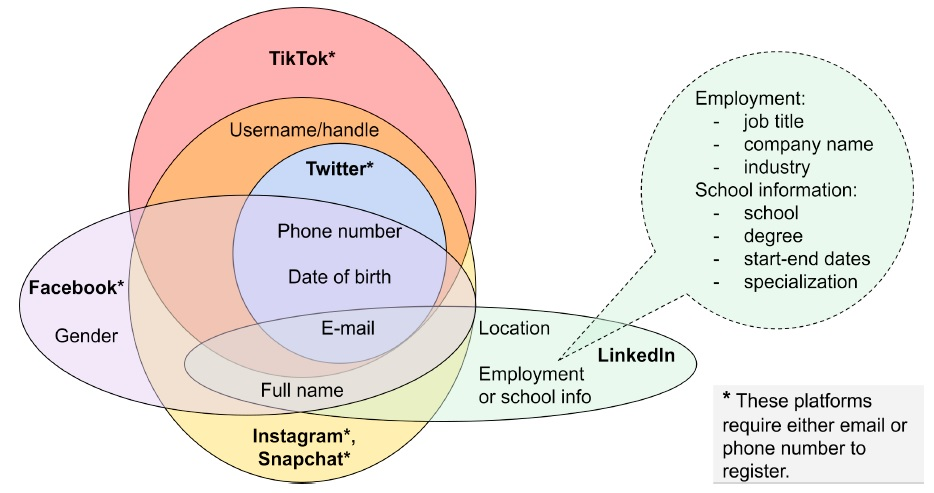
\includegraphics[width=0.7\textwidth,natwidth=650,natheight=300]{figs/req_fields1.png}
        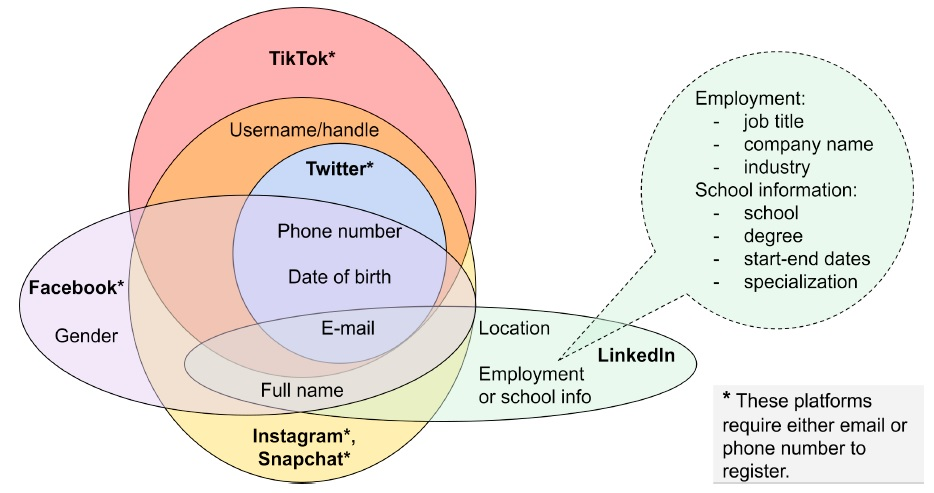
\includegraphics[width=0.7\textwidth]{figs/req_fields1.png}
    \caption{The required fields to set up an account to six popular social media platforms.}
    \label{fig:req_fields}
\end{figure}

Further, when social media data from $s_i \in \mathcal{S}$ are merged across platforms, it can lead to inferring features using $f_i$ that are not shared publicly in ${\mathcal{I}^p_i}$. These additional features may be ones that the user $u_i \in \mathcal{U}$ does not want a researcher or external entity to have. This is a privacy concern if consent is not obtained and/or the benefit of determining the value does not outweigh the harm. Also, privacy issues exist because different demographic subpopulations share attributes across multiple platforms that are more sensitive than other subpopulations, making for easier linking. This leads to a greater privacy loss for some subset of users, who perhaps may belong to more vulnerable communities.

Again, this social media challenge brings us to ethical concerns related to autonomy and justice. 
Autonomy is a concern because the more data available across sites, the more companies and others can identify and specific users. If the targeted population is a vulnerable one, issues of justice also arise. 


%\begin{table}[tb]
\begin{figure}[tb]
\small
    \caption{Optional fields for six popular social media platforms}
    \label{tab:optional}
    %    \begin{subtable}{\textwidth}
        \begin{minipage}{\textwidth}
        \centering
        \caption{Common across platforms}
        \label{tab:optional-a}
            \begin{tabular}{lcccccc} 
            \toprule
Field &   Facebook &   Instagram &   Snapchat &   Tiktok &   Twitter &   LinkedIn \\ \midrule    
Current city       & \cmark &        &  &        & \cmark & \cmark \\ \hline 
School information & \cmark &        &  &        & \cmark & \cmark \\ \hline 
Profile picture    & \cmark & \cmark &  & \cmark & \cmark & \cmark \\ \hline
Cover photo        & \cmark &        &  &        & \cmark & \cmark \\ \hline
Workplace          & \cmark &        &  &        &        & \cmark \\ \hline
Gender             & \cmark & \cmark &  &        &        &        \\ \hline
Bio                & \cmark & \cmark &  &        & \cmark & \cmark \\ \hline
Interested topic   &        &        &  &        & \cmark & \cmark \\ \hline
Website            & \cmark &        &  &        & \cmark &       \\ \bottomrule
            \end{tabular} 
            %    \end{subtable}%
    \end{minipage}%
    \vspace{1em}
%    \begin{subtable}{\textwidth}
    \begin{minipage}{\textwidth}      
        \centering
        \caption{Unique per platform}
        \label{tab:optional-b}
                             
\begin{tabular}{clclcc}
\textbf{Facebook}   &  & \textbf{Snapchat}            &  & \multicolumn{2}{c}{\textbf{LinkedIn}}    \\ \cline{1-1} \cline{3-3} \cline{5-6} 
Hometown            &  & Bitmoji (personalized emoji) &  & Licences \& certifications & Skills      \\
Relationship status &  &                              &  & List of coursework         & Patents     \\
Family members      &  & \textbf{Tiktok}              &  & Looking for a job          & Industry    \\ \cline{3-3}
                    &  & Profile video                &  & Honors \& awards           & Projects    \\
                    &  &                              &  & Volunteering               & Test scores \\
                    &  &                              &  & Publications               & Languages  
        \end{tabular} 
%    \end{subtable}
    \end{minipage}
    %\end{table}
\end{figure}

\section{Algorithmic Bias}
\label{sec:bias} 

Researchers from various fields have mined content from social media (that arises organically) to study phenomena traditionally measured using surveys. Within computer science we tend to do this without consent because we view these data as public. But we do need to pause to ask ourselves if the goal of our research is beneficial to the users, the platform, or society more broadly. Should we use such data for inference? Do users realize that their content can be used for various prediction tasks and indirect measurement of different quantities? When is it reasonable for algorithms to use knowledge about membership in a protected subpopulations to infer undisclosed attributes? What is the impact of biased algorithms on individuals? How do we begin to understand the level of harm when we do not have agreed upon ways to measure it? Fairness in machine learning and algorithmic bias are research areas that have begun thinking about some of these questions. Ultimately, using these inferences that were obtained without consent to influence a user's online behavior can be viewed as disregard for a user's actions, which conflicts with the ethical principle of \textit{respect of autonomy}. Making poor quality inferences with or without consent can increase the potential for discrimination (\textit{justice}), potentially manipulation and harm (\textit{beneficence}). When we also consider the potential harm for classes of people as opposed to just individuals, the ethical principle of \textit{societal good maximization} comes into play. We will see that these ethical principles are the primary concerns for each of the social media challenges presented in this section.

Many of the challenges in this section arise because of the differential use of social media. Social media platforms allow their users to communicate with others outside existing social and local boundaries and share with their connections user-generated content. The data generation process is not predictable across all types of users in terms of frequency, types of activity, ways of expression, or topics. People use social media differently and share different aspects of their lives. For some people social media is a social platform. For others it is a professional platform. Different types of engagement (post, comment, share, reaction, or just reading a post) can be driven by similar motivations.  

\subsection{Lack of population coverage}

Inferences from social media data are inherently of unknown representativeness because they come from nonprobability samples that are not designed to cover the population. While non-probability samples are not unique to social media, they are the norm across social media settings. Social media users $\mathcal{U}$ and the different classes/groups they form based on $c(\cdot)$ are not a representative image of the general population, limiting the direct application of many traditional techniques. For example, stratified random sampling techniques used in traditional survey methodology~\cite{deleeuw2008} cannot be directly applied without a proper sampling frame or observed characteristics to help researchers determine the strata in which different individuals fall. This is not to say that social media data are always non-representative. Social media data may end up adequately covering the research topics under study, and thus represent the population accurately, even though the individuals who contributed to the social media corpus are not sampled in a representative way~\cite{schober2016}.
Table \ref{table:platform-demographics} shows the reported populations of each of our example social media sites.  We see that levels of participation on these different sites vary with demographics. LinkedIn and Twitter have more men than women, all of the sites have larger proportions of younger users than older ones, and most have more college educated users than non-college educated.  

Being able to generalize beyond the population of a single platform is important for understanding attitudes and opinions across broader cross-sections of the population. Further, algorithms that are developed for one platform population may need to be adjusted for other populations. Without adjustments, new issues around fairness may arise. Therefore, developing methods for re-weighting populations would increase societal benefit. However, platforms do not share such data about the population distribution in sufficiently regular intervals for researchers to generalize beyond the sample they have without explicitly linking the data to a representative survey. Selection bias has been shown to reduce machine learning fairness in more traditional data sets \cite{suresh2020framework,Kamiran2011DataPT}. This type of bias is exacerbated on social media because we may be unaware of under-representation of subgroups or skews in the data since that information is not released by platforms. This could lead to socially destructive, rather than socially beneficial, knowledge production because of re-enforcement of stereotypes, bias propagation, etc. When we move to high levels of data imbalance, fairness metrics (demographic parity and equality of opportunity) get worse across all levels of privacy~\cite{farrand2020}. Finally, when demographic data is not part of the available data, we cannot verify that algorithms are being fair. As a result, extra caution is necessary when using social media data as direct \cite{de2013predicting} or indirect \cite{10.1145/3292500.3330774}  predictors of social phenomena, and why we need to help build social media benchmarks. 

Ultimately, all of these types of poor quality inferences can lead to concerns with regards to the ethical principles of justice and beneficence. 

\begin{table}[h]
\small
\centering
\caption{Percentage of U.S. adults who use each social media platform by demographics~\cite{sm_demo} }
\label{table:platform-demographics}
\begin{tabular}{cccccc}
\toprule
                      & Facebook & Instagram & LinkedIn & Twitter & Snapchat \\ \midrule
Total                 & 69\%     & 37\%      & 27\%     & 22\%    & 24\%     \\ \midrule
Men                   & 63\%     & 31\%      & 29\%     & 24\%    & 24\% \\ 
Women                 & 75\%     & 43\%      & 24\%     & 21\%    & 24\% \\ \midrule
Ages 18-29          & 79\%     & 67\%      & 28\%     & 38\%    & 62\% \\ 
30-49                 & 79\%     & 47\%      & 37\%     & 26\%    & 25\% \\ 
50-64                 & 68\%     & 23\%      & 24\%     & 17\%    & 9\% \\ 
65+                   & 46\%     & 8\%       & 11\%     & 7\%     & 3\% \\ \midrule
High school or less & 61\%     & 33\%      & 9\%      & 13\%    & 22\%       \\ 
Some college        & 75\%     & 37\%      & 26\%     & 24\%    & 29\%       \\ 
College graduate    & 74\%     & 43\%      & 51\%     & 32\%    & 20\%       \\ \bottomrule
\end{tabular}
\end{table}





\subsection{Types of Data}
Different platforms allow users to generate different types of data, including text (tweets, posts), image and video (profile image, posted photos/videos, and tagged photos/videos), geographic location (geotagged posts/tweets), and relationships/networks (friends and followers). For example, on Twitter the primary mode of communication is text. On Instagram the primary mode is images and on Tiktok the primary mode is video. 

While the prevalence of natural language processing (NLP) and text mining techniques has increased, they are less reliable on short, informal text. Many researchers are applying the same algorithms without making adjustments for the data environment, including understanding the impact of different preprocessing methods on models and adjusting the learning model to account for the noise and bias of social media data. Images have similar issues. While some images are easier to learn from, images shared on social media vary in size, format, and resolution, limiting the reliability of inferences made using these data. Ultimately, algorithms need to be designed or adjusted to compensate for new types of noise prevalent on different social media sites. 


The language used by individuals can reveal demographic characteristics and beliefs. Companies can use images to determine a user's  gender, race, and age even if the user chooses not to share this information. Companies can use geolocation to get user's location and use the location to predict certain characteristics (such as age, gender and income) or even, predict where a user lives or works. For example, researchers have used Twitter user descriptions to infer consumer profiles, predicting attributes such as parental status or if the user is a frequent traveler from the textual content with a precision of between $80\%$ and $92\%$~\cite{hernandez2013}. They also used textual clues, mentions of regional events, Foursquare check-ins, geo-tagged messages, and time zone settings to infer user location with high precision. 

Only recently have researchers begun considering the social impact of natural language processing (NLP)~\cite{hovy2016,blodgett2020}. Text in posts capture how we express ourselves, and they can also capture historical biases and propagate them in the models built~\cite{garg2018,caliskan2017}. For example, word embeddings have been shown to inherit gender bias~\cite{sun2019,bolukbasi2016a,gonen2019}. Additionally, NLP techniques can have difficulty understanding specific dialects within a language~\cite{blodgett2016}. As a result, in the context of social media, dialect speakers’ opinions may be mischaracterized. This is particularly applicable for applications using sentiment analysis and stance. In this context, dialect speakers are discriminated against and possibly even excluded from these models, leading to clear conflicts with regards to the ethical principles of \textit{justice} and \textit{societal good maximisation}\cite{mikal2016}.


\subsection{Sensitive data}
Advances in machine learning have made it possible to infer a large range of attributes about a person. For example, just using information shared in posts, algorithms can infer gender, age, and location with high accuracy.  And when sensitive data are available, e.g. birthdate or race, they will tend to lead to stronger inference predictions. Using these sensitive data for prediction violate the anti-classification definition of fairness, which states that sensitive attributes should not be part of the data used to get a model's outcome. However, an important use of this sensitive information is to ensure group-level and individual-level fairness. 

Because non-sensitive shared personal data of a user or the user's friends can serve as indirect indicator of the user's demographic information, as researchers of data-driven systems, we need to integrate methods to ensure that features generated from personal data are not biased. Additionally, models that do not use sensitive information might still exhibit indirect discrimination, as non-protected attributes may correlate with the protected ones. This is referred to as the ``red-lining'' effect. 

These concerns bring up issues related to the ethical principles of justice and maximizing social benefit. There are many examples of indirect discrimination \cite{oneil2016}. For example, the LinkedIn talent search system returns a list of candidates based on a search query. The system was found to be biased against race and gender and has since been updated \cite{linkedin_unfair}. Another example is Amazon's 2014 hiring application that reviewed resumes to identify top candidates for interviewing. The algorithm was found to be biased against females because the training data (current employee resumes) was heavily biased towards men. Different resume attributes that were being learned by the algorithm were serving as indirect indicators of gender~\cite{dastin_2018}.
These examples are a reminder of the impact of historical data on propagating present day bias. It arises when there is a misalignment between the world as it is and the values or objectives that are encoded and propagated in a model. This bias refers to a concern with the state of the world, and care must be given to this issue on social media, where organic data has inherent biases. If researchers do not correct the biases present in the organic data, they will replicate those biases in the findings, further reinforcing social and cultural inequities. 


\subsection{Partial Information Sharing - Missing data}
People do not fill out all the fields when they sign up for a social media account, revealing different amounts of personal information to others.  Some express their opinions about a larger range of topics than others. Users may share different information with their private network than on their public profile. Ultimately, other than required fields and auto-generated fields, there are very few pieces of information that can be directly obtained across all of the users (see Table \ref{tab:optional}). The result is a significant amount of missing data. 

It is not surprising that companies and researchers have attempted to infer this missing information. However, what happens if the inferred value is incorrect and that value is assumed as accurate for another algorithm? When the data are representative and the algorithms are accurate, the inferences may benefit users. When they are inaccurate and this inaccuracy is further propagated in other algorithms, the harm can be significant.  

The impact of missing values on fairness can be significant. If users choose to not share certain demographic information, how can researchers test if a model is biased against this individual? If we do not have ground truth about the users' sensitive information/features, we cannot verify and guarantee that any models built or conclusions drawn are not biased against (or favoring) a specific set of users. This can be especially problematic when the classification outcome is dependent on users' known features, and these features are correlated to sensitive attributes that are missing. In order to overcome this challenge, some recent research has focused on a pre-processing stage that attempts to ensure that user representation does not indirectly carry any demographic information \cite{10.1177/2053951717743530,Kamiran2011DataPT}. Developing new approaches for measuring fairness when the properties of the underlying data are only partially known is particularly important for social media.

Finally, more generally, we cannot ignore the role missing information plays within data mining and machine learning methods that are deployed on social media.  If missing values are in non-sensitive features, and if the missing values are completely at random, the models being built should be robust. However, if the missing values show bias by exhibiting specific patterns, the models using these data will also be biased \cite{little2019statistical}, raising concerns associated with the ethical principle of justice. 

\subsection{Imbalanced levels of activity}
Users on social media are not equally active. Some are very active, posting continually, while others only browse channels of interest. For example, on Twitter, the top 10\% of the most active tweeters by number of tweets are responsible for 80\% of all tweets created by U.S. adults \cite{pew_twitter}. Levels of engagement can also vary with demographics, campaigns, and across platforms~\cite{perrin2019}. Popular profiles that have many followers/likes tend to post more often than the rest. Figure~\ref{fig:mins_per_day} shows the amount of time users spend on different platforms. While these numbers continues to rise, they vary considerably by demographic. For example, while adults in the US average 38 minutes on Facebook per day, those of ages 16-24 spend three hours on the platform~\cite{whatagraph2020}. Globally, people spent 144 minutes per day on social media. In the United States, people spent 123 minutes per day on social media~\cite{sm_usage}, while they only spent 19 minutes per day exercising~\cite{american_time_spent2020}. In other words, many people are very inclined to spend more time on social media than certain other leisure activity, allowing for potentially better quality inferences; however, the variability is large, requiring researchers to ensure sufficient data are available for stable, repeatable algorithmic development. 
\begin{figure}
    \centering
    %    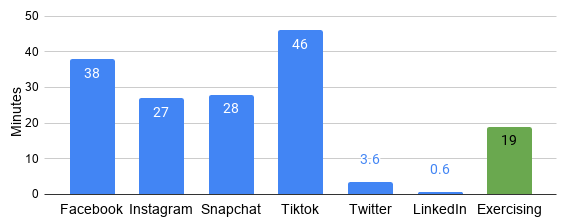
\includegraphics[width=10cm,height = 2cm,natwidth=420,natheight=100]{figs/time_spentExercise.png}
        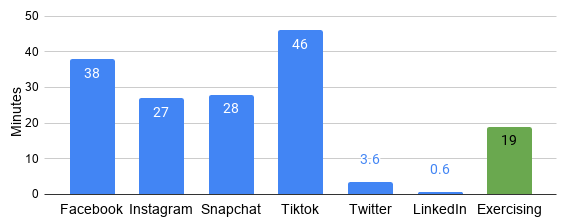
\includegraphics[width=10cm,height = 2cm]{figs/time_spentExercise.png}
    \caption{Average time people spent on each social media platform per day (in minutes).} 
    \label{fig:mins_per_day}
\end{figure}


Also, sometimes researchers only have posts from a particular group or channel and do not know the overall activity level of the users posting on the channel. If the inference is about the content of the post itself, that can be reliable. However, when companies and researchers make inferences about the users, they need to determine the minimum number of posts needed per user for the task. Not doing so will not only lead to measurement validity issues, but also algorithmic bias issues, where accuracy will be higher for those who are more active on social media. Ignoring the levels of user activity when building models reduces the fairness of the model. Inferences made on individuals who post less frequently are likely to be less reliable and more prone to measurement bias, leading to concerns associated with the ethical considerations of non-maleficence and justice.

\section{Transparent Computing}
\label{sec:transparency}
Users are inundated with huge volumes of information and a large number of choices. Social media applications have only made this more challenging. Users may be unaware of the data that are being shared or used by different platforms, and if they are aware, they may not understand how the platforms are using the data or how to make adjustments to their data sharing preferences. For example, many users on Facebook are not aware that people outside of their network of friends can see their account information \cite{orito_2014,FB_targetad}.
At the same time, computational models continue to increase in complexity, making it harder for researchers and programmers to understand the impact of different data features on developed inference models. 

As machine learning models continue to influence human behavior and drive our decision making, the topic of transparency continues to reoccur within this context. Transparency is being discussed as a synonym for interpretability, i.e. an explanation of the model, to ensure a model's outcomes are understandable and fair to humans. However, transparent/interpretable models are only one piece of the learning process, or more broadly, of a computational model. Algorithmic fairness and privacy capture important desired characteristics of an implemented computing model with respect to ethical concerns. However, we argue that these concepts capture only a part of computational transparency. The complexity of the data and the software require use to to reimagine data and software transparency. This includes transparency during data collection, data preprocessing, model design and implementation, and model outputs.  When a system and the data within the system are transparent across all its components, it is not only easier to understand the system, but it also makes it easier to determine the components most vulnerable to ethical attacks. 

Having more transparency throughout the software development lifecycle is not a new idea. However, exposing both the inputs and the data usages throughout will enable researchers to connect computation to the ethical principles defined in Section \ref{sec:ethics}. Toward that end, we define \textit{transparent computing} to be the study of transparency mechanisms for computing. Transparency is fundamental to all of the mentioned ethical principles. The pillars of transparent computing would include the following: (1) ensuring that coded policy constraints, including ethical considerations, related to user data are transparent, (2) ensuring that the data being used by algorithms are transparent,\footnote{In cases where data values cannot be shared, measures can be shared to inform researchers about the properties of the data.} (3) ensuring that the models used to make inferences are transparent, and when possible interpretable, (4) ensuring that the reliability of the algorithm in terms of accuracy and fairness are transparent, and (5) ensuring that generalizability and limitations of model usage and analysis are clear. Without embedding principles of transparency into our problem formulation, model construction, and shared results, quantifying and measuring the effectiveness of our algorithms and privacy mechanisms with regards to ethical principles will not be straightforward. Our field will continue to have to grapple with the inconsistency between what we do and what makes ethical sense to do.

\section{Final Thoughts}
While some of the complexities we identify are are not novel and have been issues associated with traditional data sources, e.g. surveys and administrative data, the social media context is new and requires us to rethink our approach for addressing these complexities, while understanding the ethical implications of our solutions. 
%Given the complexities specific to social media, what are the ethical conundrums that are emerging as they relate to algorithmic bias and data privacy? 
How do we ensure that algorithms and tools that we design are fair, transparent, and privacy preserving to humans, while also being beneficial to society? The irregular noise in social media data, the inherent bias in features generated from the data, and the lack of understanding of the representativeness of social media platforms make it harder to develop correct and sound algorithmic, machine learning, and privacy solutions. And that difficulty is even more challenging when we throw ethics into the mix. As computer science researchers, we are at an important crossroad. We can continue to build algorithms and tools that companies use to exploit user data. Or we can understand that users who share their data freely with companies need researchers to develop guidelines for use of these data, for design of algorithms that consider transparency and fairness, and for technologies that protect user data and use user data responsibly. 

While this area is emerging and guidelines are still be developed, there are best practices that have been identified in other disciplines that we can begin to follow. First, if possible, researchers should use public data and make clear in the study how the data are collected. If the data are private, researchers can conduct thought exercises that work through the potential ethical considerations and potential user/societal harms to ensure that the use of private data is warranted. If a decision is made to move forward, the researchers should get consent to use the data and give users options to decline and leave the study at any point. When inferring new values or developing new models, researchers can compute not only measures of accuracy, but also measures of fairness. Finally, researchers should continue to make data, models, and results transparent and reproducible. By designing algorithms and technologies with ethical considerations from the outset, perhaps we can begin to create a new breed of computer science that deliberately connects our computation work to social responsibility.
\section*{Acknowledgements}
This research is funded by National Science Foundation awards \#1934925 and \#1934494, the National Collaborative on Gun Violence Research (NCGVR), the Fritz Family Fellowship, and the Massive Data Institute (MDI) at Georgetown University. We thank our funders for supporting this research. 

\begin{thebibliography}{10}
\begin{small}
\itemsep=1pt


\bibitem{american_time_spent2020}
American {Time} {U}se {S}urvey {News} {Release} - 2019 {Results} (2020),
  https://www.bls.gov/news.release/archives/atus \_06252020.htm

\bibitem{bagrow2019}
Bagrow, J.P., Liu, X., Mitchell, L.: Information flow reveals prediction limits
  in online social activity. Nature Human Behaviour  \textbf{3}(2),  122--128
  (Feb 2019)

\bibitem{barth2017}
Barth, S., De~Jong, M.D.: The privacy paradox--{Investigating} discrepancies
  between expressed privacy concerns and actual online behavior–{A}
  systematic literature review. Telematics and informatics  \textbf{34}(7),
  1038--1058 (2017)

\bibitem{blodgett2020}
Blodgett, S.L., Barocas, S., Daumé~III, H., Wallach, H.: Language
  ({Technology}) is {Power}: {A} {Critical} {Survey} of  ``{Bias}" in {NLP}.
  arXiv preprint arXiv:2005.14050  (2020)

\bibitem{blodgett2016}
Blodgett, S.L., Green, L., O'Connor, B.: Demographic dialectal variation in
  social media: {A} case study of {African}-{American} {English}. arXiv
  preprint arXiv:1608.08868  (2016)

\bibitem{bolukbasi2016a}
Bolukbasi, T., Chang, K.W., Zou, J.Y., Saligrama, V., Kalai, A.T.: Man is to
  computer programmer as woman is to homemaker? debiasing word embeddings. In:
  Advances in neural information processing systems (2016)

\bibitem{caliskan2017}
Caliskan, A., Bryson, J.J., Narayanan, A.: Semantics derived automatically from
  language corpora contain human-like biases. Science  \textbf{356}(6334),
  183--186 (2017)

\bibitem{10.1145/3376898}
Chouldechova, A., Roth, A.: A snapshot of the frontiers of fairness in machine
  learning. Commun. ACM  \textbf{63}(5),  82-89 (Apr 2020)

\bibitem{dastin_2018}
Dastin, J.: Amazon scraps secret ai recruiting tool that showed bias against
  women (2018),
  https://www.reuters.com/article/us-amazon-com-jobs-automation-insight/amazon-scraps-secret-ai-recruiting-tool-that-showed-bias-against-women-idUSKCN1MK08G

\bibitem{linkedin_unfair}
Day, M.: How linkedin's search engine may reflect a gender bias (Aug 2016),
  https://www.seattletimes.com/business/microsoft/how-linkedins-search-engine-may-reflect-a-bias

\bibitem{de2013predicting}
De~Choudhury, M., Gamon, M., Counts, S., Horvitz, E.: Predicting depression via
  social media. Icwsm  \textbf{13},  1--10 (2013)

\bibitem{deleeuw2008}
De~Leeuw, E.D., Hox, J.J., Dillman, D.A.: International handbook of survey
  methodology. Taylor \& Francis Group/Lawrence Erlbaum Associates (2008)

\bibitem{farrand2020}
Farrand, T., Mireshghallah, F., Singh, S., Trask, A.: Neither private nor fair:
  Impact of data imbalance on utility and fairness in differential privacy.
  arXiv preprint arXiv:2009.06389  (2020)

\bibitem{garg2018}
Garg, N., Schiebinger, L., Jurafsky, D., Zou, J.: Word embeddings quantify 100
  years of gender and ethnic stereotypes. Proceedings of the National Academy
  of Sciences  \textbf{115}(16),  E3635--E3644 (2018)

\bibitem{gonen2019}
Gonen, H., Goldberg, Y.: Lipstick on a pig: {Debiasing} methods cover up
  systematic gender biases in word embeddings but do not remove them. arXiv
  preprint arXiv:1903.03862  (2019)

\bibitem{us1979belmont}
of~Health, U.D., Services, H., et~al.: The belmont report: Office of the
  secretary, ethical principles and guidelines for the protection of human
  subjects of research, the national commission for the protection of human
  subjects of biomedical and behavioral research (1979)

\bibitem{sm_usage}
Henderson, G.: How much time does the average person spend on social media?
  (Aug 2020),
  https://www.digitalmarketing.org/blog/how-much-time-does-the-average-person-spend-on-social-media

\bibitem{hernandez2013}
Hernandez, M., Hildrum, K., Jain, P., Wagle, R., Alexe, B., Krishnamurthy, R.,
  Stanoi, I.R., Venkatramani, C.: Constructing consumer profiles from social
  media data. In: {IEEE} {International} {Conference} on {Big} {Data}. pp.
  710--716. IEEE (2013)

\bibitem{FB_targetad}
Hitlin, P., Rainie, L.: Facebook algorithms and personal data (Jan 2019),
  https://www.pewresearch.org/internet/2019/01/16/facebook-algorithms-and-personal-data/

\bibitem{hovy2016}
Hovy, D., Spruit, S.L.: The social impact of natural language processing. In:
  Proceedings of the 54th {Annual} {Meeting} of the {Association} for
  {Computational} {Linguistics} ({Volume} 2: {Short} {Papers}). pp. 591--598
  (2016)

\bibitem{pew_twitter}
Hughes, A., Wojcik, S.: Key takeaways from our new study of how americans use
  twitter (April 2019),
  https://www.pewresearch.org/fact-tank/2019/04/24/key-takeaways-from-our-new-study-of-how-americans-use-twitter

\bibitem{Kamiran2011DataPT}
Kamiran, F., Calders, T.: Data preprocessing techniques for classification
  without discrimination. Knowledge and Information Systems  \textbf{33},
  1--33 (2011)

\bibitem{kammourieh2017}
Kammourieh, L., Baar, T., Berens, J., Letouzé, E., Manske, J., Palmer, J.,
  Sangokoya, D., Vinck, P.: Group privacy in the age of big data. In: Group
  {Privacy}, pp. 37--66. Springer (2017)

\bibitem{kokolakis2017}
Kokolakis, S.: Privacy attitudes and privacy behaviour: {A} review of current
  research on the privacy paradox phenomenon. Computers \& security
  \textbf{64},  122--134 (2017)

\bibitem{Kramer8788}
Kramer, A.D.I., Guillory, J.E., Hancock, J.T.: Experimental evidence of
  massive-scale emotional contagion through social networks. Proceedings of the
  National Academy of Sciences  \textbf{111}(24),  8788--8790 (2014)

\bibitem{Lipworth2017}
Lipworth, W., Mason, P., Kerridge, I., Ioannidis, J.: Ethics and epistemology
  in big data research. Journal of Bioethical Inquiry  \textbf{14} (2017)

\bibitem{little2019statistical}
Little, R.J., Rubin, D.B.: Statistical analysis with missing data, vol.~793.
  John Wiley \& Sons (2019)

\bibitem{luka2017}
Luka, M.E., Millette, M., Wallace, J.: A feminist perspective on ethical
  digital methods. Internet research ethics for the social age p.~21 (2017)

\bibitem{10.1080/15265161.2019.1602190}
Lynch, H.F., Largent, E.A.: Mountains and molehills when using social media as
  a research support tool. The American Journal of Bioethics  \textbf{19}(6),
  64--66 (2019)

\bibitem{madden2013teens}
Madden, M., Lenhart, A., Cortesi, S., Gasser, U., Duggan, M., Smith, A.,
  Beaton, M.: Teens, social media, and privacy. Pew Research Center
  \textbf{21}(1055),  2--86 (2013)

\bibitem{mikal2016}
Mikal, J., Hurst, S., Conway, M.: Ethical issues in using {Twitter} for
  population-level depression monitoring: a qualitative study. BMC medical
  ethics  \textbf{17}(1), ~22 (2016)

\bibitem{7515114}
{O'Leary}, D.E.: Ethics for big data and analytics. IEEE Intelligent Systems
  \textbf{31}(4),  81--84 (2016)

\bibitem{oneil2016}
O'neil, C.: Weapons of math destruction: How big data increases inequality and
  threatens democracy. Broadway Books (2016)

\bibitem{orito_2014}
Orito, Y., Fukuta, Y., Murata, K.: I will continue to use this nonetheless:
  Social media survive users' privacy concerns. International Journal of
  Virtual Worlds and Human Computer Interaction  \textbf{2},  92--107 (12 2014)

\bibitem{socialdilemma}
Orlowski, J.: The social dilemma. Exposure Labs (2020)

\bibitem{smconcern}
Perrin, A.: Americans are changing their relationship with facebook (Sep 2018),
  https://www.pewresearch.org/fact-tank/2018/09/05/americans-are-changing-their-relationship-with-facebook/

\bibitem{perrin2019}
Perrin, A., Andreson, M.: Share of {U}.{S}. adults using social media,
  including {Facebook}, is mostly unchanged since 2018 (Apr 2019),
  https://www.pewresearch.org/fact-tank/2019/04/10/share-of-u-s-adults-using-social-media-including-facebook-is-mostly-unchanged-since-2018/

\bibitem{sm_demo}
Social media fact sheet (Jun 2019),
  https://www.pewresearch.org/internet/fact-sheet/social-media/

\bibitem{10.1177/1556264619901215}
Samuel, G., Buchanan, E.: Guest editorial: Ethical issues in social media
  research. Journal of Empirical Research on Human Research Ethics
  \textbf{15}(1-2),  3--11 (2020)

\bibitem{samuel2019}
Samuel, G., Derrick, G.E., van Leeuwen, T.: The {Ethics} {Ecosystem}:
  {Personal} {Ethics}, {Network} {Governance} and {Regulating} {Actors}
  {Governing} the {Use} of {Social} {Media} {Research} {Data}. Minerva
  \textbf{57}(3),  317--343 (Sep 2019)

\bibitem{schober2016}
Schober, M.F., Pasek, J., Guggenheim, L., Lampe, C., Conrad, F.G.: Social
  {Media} {Analyses} for {Social} {Measurement}. Public Opinion Quarterly
  \textbf{80}(1),  180--211 (2016)

\bibitem{SENTHILKUMARN2016114}
{Senthil Kumar N}, {Saravanakumar K}, {Deepa K}: On privacy and security in
  social media : A comprehensive study. Procedia Computer Science  \textbf{78},
   114 -- 119 (2016), international Conference on Information Security \&
  Privacy 2015

\bibitem{10.1145/3068777.3068781}
Shu, K., Wang, S., Tang, J., Zafarani, R., Liu, H.: User identity linkage
  across online social networks: A review. SIGKDD Explor. Newsl.
  \textbf{18}(2),  5–17 (Mar 2017)

\bibitem{10.1145/3292500.3330774}
Singh, L., Wahedi, L., Wang, Y., Wei, Y., Kirov, C., Martin, S., Donato, K.,
  Liu, Y., Kawintiranon, K.: Blending noisy social media signals with
  traditional movement variables to predict forced migration. p. 1975–1983.
  KDD '19, Association for Computing Machinery, New York, NY, USA (2019)

\bibitem{singh2015}
Singh, L., Yang, G.H., Sherr, M., Hian{-}Cheong, A., Tian, K., Zhu, J., Zhang,
  S.: Public information exposure detection: Helping users understand their web
  footprints. In: {IEEE/ACM} International Conference on Advances in Social
  Networks Analysis and Mining (ASONAM). pp. 153--161. Paris, France (August
  2015)

\bibitem{smconcern1}
New duckduckgo research shows people taking action on privacy (Oct 2019),
  https://spreadprivacy.com/people-taking-action-on-privacy/

\bibitem{sun2019}
Sun, T., Gaut, A., Tang, S., Huang, Y., ElSherief, M., Zhao, J., Mirza, D.,
  Belding, E., Chang, K.W., Wang, W.Y.: Mitigating gender bias in natural
  language processing: {Literature} review. arXiv preprint arXiv:1906.08976
  (2019)

\bibitem{suresh2020framework}
Suresh, H., Guttag, J.V.: A framework for understanding unintended consequences
  of machine learning (2020)

\bibitem{b88a5a9441354a02ac5b105291fff917}
Susser, D.: Information privacy and social self-authorship. Techne: Research in
  Philosophy and Technology  \textbf{20}(3),  216--239 (2016), copyright:
  Copyright 2017 Elsevier B.V., All rights reserved.

\bibitem{Susser2018}
Susser, D., Roessler, B., Nissenbaum, H.: Online manipulation: Hidden
  influences in a digital world. SSRN Electronic Journal  (01 2018)

\bibitem{TANGWA2009S2}
Tangwa, G.B.: Ethical principles in health research and review process. Acta
  Tropica  \textbf{112},  S2 -- S7 (2009), health Research in Africa: Ethical
  and Practical Challenges

\bibitem{10.1177/1747016117738559}
Taylor, J., Pagliari, C.: Mining social media data: How are research sponsors
  and researchers addressing the ethical challenges? Research Ethics
  \textbf{14}(2),  1--39 (2018)

\bibitem{thaler2009}
Thaler, R.H., Sunstein, C.R.: Nudge: Improving decisions about health, wealth,
  and happiness. Penguin (2009)

\bibitem{10.1080/15265161.2019.1611278}
Torous, J., Ungar, L., Barnett, I.: Expanding, augmenting, and operationalizing
  ethical and regulatory considerations for using social media platforms in
  research and health care. The American Journal of Bioethics  \textbf{19}(6),
  ~4--6 (2019)

\bibitem{Turoldo2008}
Turoldo, F.: Responsibility as an ethical framework for public health
  interventions. American journal of public health  \textbf{99},  1197--202 (11
  2008)

\bibitem{10.1177/2053951717743530}
Veale, M., Binns, R.: Fairer machine learning in the real world: Mitigating
  discrimination without collecting sensitive data. Big Data \& Society
  \textbf{4}(2),  2053951717743530 (2017)

\bibitem{fb_Analytica}
Wagner, K.: Here’s how facebook allowed cambridge analytica to get data for
  50 million users (Mar 2018),
  https://www.vox.com/2018/3/17/17134072/facebook-cambridge-analytica-trump-explained-user-data

\bibitem{whatagraph2020}
How much time do people spend on social media (11 insights) {\textbar} {Blog}
  {\textbar} {Whatagraph} (Aug 2020),
  https://whatagraph.com/blog/articles/how-much-time-do-people-spend-on-social-media

\bibitem{ozkula2020}
Özkula, S.M.: The {Issue} of ``{Context}": {Data}, {Culture}, and
  {Commercial} {Context} in {Social} {Media} {Ethics}. Journal of Empirical
  Research on Human Research Ethics  \textbf{15}(1-2),  77--86 (2020)
\end{small}
\end{thebibliography}

%
% BibTeX users please use
% \bibliographystyle{}
% \bibliography{}


\end{document}




